\section{Using \dReach{}}\label{sec:using-dreach}

We now describe the input format and command line options of \dReach{}.

\subsection{Input Format}\label{sec:input-format}

\begin{figure}
  \begin{framed}
    % drh
    \begin{align*}
      \textit{drh} := \ & \textit{macro-definition}^* \ \textit{variable-declaration}^+ \\
                        & \textit{mode-definition}^+ \  \textit{initial-condition} \  \textit{goal}^+\\
    % variable-decl
      \textit{macro-declaration} \ := \ &  \texttt{\#define} \ \textit{var} \ (\textit{expr} \, | \, \textit{formula})\\
    % variable-decl
      \textit{variable-declaration} \ := \ &  \texttt{[}
                                              \textit{l}
                                              \texttt{,}
                                              \ \textit{u}
                                              \texttt{]}
                                              \ \textit{var}
                                              \texttt{;}\\
    % variable-decl
      \textit{mode-definition} \ := \ & \ \texttt{\{}
                                         \texttt{mode} \
                                         \textit{id}\texttt{;} \quad
                                         \texttt{invt}:(\textit{formula} \texttt{;})^+\\
                                    & \ \ \ \texttt{flow}:\textit{ode}^+ \quad
                                    \texttt{jump}:\textit{jump}^+ \texttt{\}}\\
      \textit{ode} \ := \ & \texttt{d/dt[}\textit{x}\texttt{]=}\textit{exp}\\
      \textit{jump} \ := \ & \textit{formula} \ \texttt{==>} \ \texttt{@}\textit{n} \ \textit{formula}\\
      \textit{initial-condition} \ := \ & \texttt{@}\textit{mode-id} \ \textit{formula}\texttt{;}\\
      \textit{goal}              \ := \ & \texttt{@}\textit{mode-id} \ \textit{formula}\texttt{;}
    \end{align*}
  \end{framed}
  \caption{Syntax grammar of $\drh{}$}\label{fig:drh-grammar}
\end{figure}

Figure~\ref{fig:drh-grammar} describes the input language \drh{} for
describing hybrid systems and specifying reachability properties. It
consists of five sections - macro definitions, variable declarations,
mode definitions, and initial condition, and goals.

% extracted to the grammar
In macro definitions, it allows users to define macros in C
preprocessor (\texttt{cpp}) style which can be used in the following
sections. Note that macro expansions occur before the other parts are
processed.

A variable declaration specifies a real variable, $var$ and its domain
$[l, u]$ which is in Real interval $\mathbb{IR}$. \drh{} requires a
special declaration for \textit{time} variable, to specify the
upperbound of time duration in the analysis of bounded
$\delta$-reachability.

A mode definition consists of mode id, mode invariant, flow, and jump.
\textit{id} is a unique positive interger assigned to a mode. An
invariant is a conjuction of logic formulae which must always hold in
a mode. A flow describes a continuous dynamics of a mode by providing
a set of ordinary differential equations (\textit{ode}s). The first
formula of \textit{jump} is interpreted as a guard, a logic formula
specifying a condition to make a transition. Note that this allows a
transition but does not force it. The second argument of
\textit{jump}, $n$ denotes the target mode-id. The last one is
\textit{reset}, a logic formula connecting the old and new values for
the transition.

\textit{initial-condition} specifies the initial mode of a hybrid
system and its initial configuration. \textit{goal} shares the same
syntactic structure of \textit{initial-condition}. It poses a
reachability question: ``Is there a trajectory of a hybrid system
reaching \textit{mode-id} while satisfying the goal condition
\textit{formula}?''.

\begin{figure}
  \centering
  \begin{Verbatim}[fontfamily=courier, frame=single, framesep=1mm,
  numbers=left, fontsize=\scriptsize]
#define D 0.45
#define K 0.9
[0, 15] x;
[9.8] g;
[-18, 18] v;
[0, 3] time;
{   mode 1;
    invt: (v <= 0);  (x >= 0);
   flow: d/dt[x] = v;
          d/dt[v] = -g - (D * v ^ 2);
    jump: (x = 0) ==> @2 (and (x' = x) (v' = - K * v)); }
 {  mode 2;
    invt: (v >= 0); (x >= 0);
    flow: d/dt[x] = v;
          d/dt[v] = -g + (D * v ^ 2);
    jump: (v = 0) ==> @1 (and (x' = x) (v' = v)); }
init: @1 (and (x >= 5) (v = 0));
goal: @1 (and (x >= 0.45));
\end{Verbatim}
\caption{An example of \drh{} format: Inelastic bouncing ball with air
  resistance. At lines 1 and 2, we define a drag coefficient $D = 0.45$
  and an elastic coefficient $K = 0.9$ using \texttt{\#define} macros.
  At lines 3 - 6, we declare variables $x, g, v,$ and $time$. At lines
  7 - 15 and 16 - 24, we define two modes -- the falling and the
  bouncing-back modes respectively. At lines 25 and 26, we specify
  that this hybrid system starts at mode 1 (\texttt{@1}) with initial
  condition satisfying $x \ge 5 \land v = 0$. At lines 28 and 29, it
  is asking whether we can have a trajectory ending at mode 1
  (\texttt{@1}) while the height of the ball is higher than $0.45$.}
\label{fig:bouncing-ball-drh}
\end{figure}

Figure~\ref{fig:bouncing-ball-drh} shows a canonical example of hybrid
systems, an inelastic bouncing ball with air resistance, in \drh{}
format.

\subsection{Command Line Options}

\begin{Verbatim}[fontfamily=courier, frame=single, framesep=1mm, fontsize=\scriptsize]
  usage: /home/soonhok/work/dreal/bin/dReach options <*.drh> <options to dReal>

  dReach: Bounded Model Checking for for Nonlinear Hybrid Systems

  OPTIONS:
  -k   unrolling steps  (default: 3)
  -b   use BMC heuristic with disjunctive path encoding
  -r   -b and filter unreachable modes from SMT encoding
  -e   -r and filter continuous variables from SMT encoding
  -d   disjunctive path encoding

  EXAMPLE:

  dReach -k 10 bouncing_ball.drh --verbose --precision=0.001 --visualize

\end{Verbatim}

\begin{figure}
  \centering
  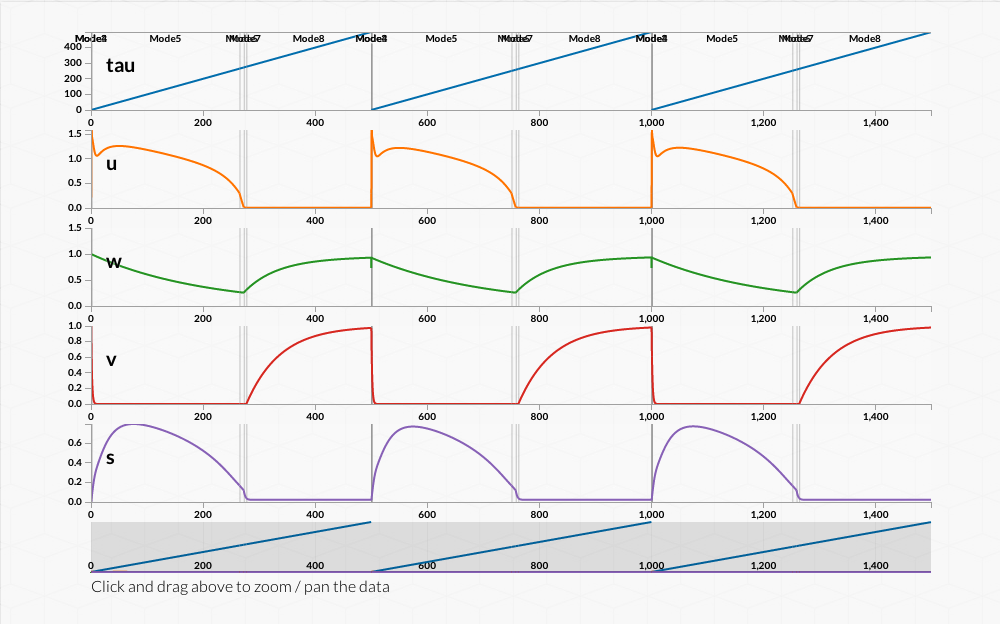
\includegraphics[width=\textwidth]{images/cardiac}
  \caption{Visualization of $\delta$-reachable trajectory for
    a cardiac-cell model.}
  \label{fig:viz}
\end{figure}


%%% Local Variables:
%%% mode: latex
%%% TeX-master: "main"
%%% End:
